\chapter{Der Large Hadron Collider und der LHCb-Detektor}
\label{chap:3}
%
\section{Der Large Hadron Collider}
%
Der \textit{Large Hadron Collider} (LHC) \cite{lhc} am CERN ist der derzeit leistungsstärkste Teilchenbeschleuniger der Welt. Er dient der Erzeugung von Proton-Proton-Kollisionen ($pp$-Kollisionen), sowie weiteren Teilchenkollisionen bei einer Schwerpunktenergie von bis zu $\sqrt{s}=\SI{14}{\tera\electronvolt}$ \cite{lhc}. Diese durch Größe und Bauteile beschränkten Energien werden nach dem letzten Upgrade mit $\SI{13}{\tera\electronvolt}$ beinahe ausgereizt \cite{lhc}. Durch die Ausweitung des zu untersuchenden Energiebereiches auf diese Größenordnung eignet sich der LHC zur Entdeckung von Physik jenseits des SM, wie etwa unbekannter Teilchen. Im Jahre 2012 gelang der ATLAS- und der CMS-Kollaboration die Entdeckung des in den 60er-Jahren von Higgs, Englert und Brout vorhergesagten Higgs-Bosons \cite{higgs_atlas, higgs_cms}.\\
Bevor die Protonen im 50 bis $\SI{175}{\meter}$ \cite{lhc} unter der Erde liegenden, $\SI{27}{\kilo\meter}$ langen Speicherring auf die maximale Schwerpunktsenergie beschleunigt werden, durchlaufen sie ein vielschrittiges System aus Vorbeschleunigern. Dessen letzte Stufe ist der \textit{Super Proton Synchrotron} (SPS), welcher die Protonen auf etwa $\SI{99,99978}{\percent}$ der Lichtgeschwindigkeit beschleunigt \cite{lhc}. Diese Protonen werden mit einer Schwerpunktsenergie von $\SI{0,45}{\tera\electronvolt}$ über zwei Transferlinien in den LHC injiziert, wo sie in entgegengesetzter Richtung beschleunigt werden. Die Beschleunigung und Kreisführung findet dabei in einem Ultrahochvakuum über \textit{radio frequency}-Kavitäten und supraleitende Magnete, welche von flüssigem Helium auf etwa $\SI{1,9}{\kelvin}$ gekühlt werden, statt. So werden Hunderte einzelner Protonenbündel auf beinahe Lichtgeschwindigkeit beschleunigt und anschließend in Abständen von $\SI{25}{\nano\second}$
($\SI{40}{\mega\hertz}$) in einem der vier großen Experimente durch Strahlkreuzung zur Kollision gebracht. Da Datenmengen in dieser Größenordnung nicht gespeichert werden können, wird ein mehrstufiges Filtersystem angewendet: die Trigger. Diese sind in drei Stufen aufgeteilt. Der Hardwaretrigger \textsc{L0} trifft direkt bei der Messung in Echtzeit Entscheidungen, sodass die Ereignisrate ein prozessierbares Niveau ($\SI{1}{\mega\hertz}$) \cite{Tilburg} erreicht, gleichzeitig aber möglichst viele Ereignisse, die potenziell physikalisch relevant sind, aufgenommen werden. Dazu werden Daten aus den Kalorimetern, sowie den Myonkammern zur Bestimmung hoher Transversalimpulse bzw. Energien verwendet. Die Softwaretrigger (\textsc{HLT1} und \textsc{HLT2}) reduzieren kurz darauf die Datensätze auf physikalisch Relevantes. Der HLT1-Trigger führt dabei eine partielle Rekonstruktion der Events über Vertex- und Spurbestimmungen durch. Der HLT2-Trigger stellt die letzte Stufe dar und kann Entscheidungen auf Grundlage der gesamten Ereignis-Informationen treffen. So wird die Datenrate von $\SI{16}{\mega\hertz}$ auf etwa $\SI{2}{\kilo\hertz}$ reduziert.
%
\section{Der LHCb Detektor}
%
\begin{figure}[H]
  \centering
      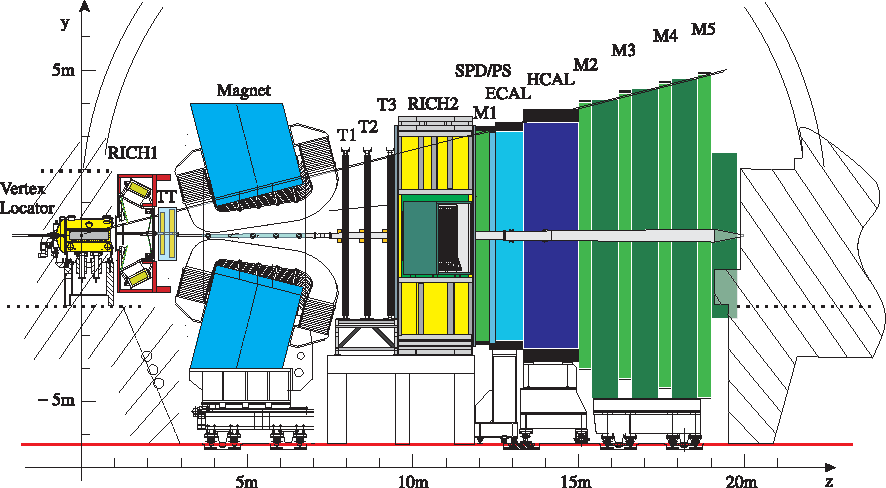
\includegraphics[width=0.89\textwidth]{Plots/lhcb.pdf}
  \caption{Querschnitt des LHCb-Detektors \cite{lhcb}.}
  \label{fig:lhcb}
\end{figure}
%
Der LHCb-Detektor deckt im Gegensatz zu den anderen drei Experimenten am LHC bei seinen Messungen nicht den gesamten Raumwinkel um den Kollisionspunkt ab. Es handelt sich hierbei um einen einarmigen vom Kollisionspunkt in einer der Strahlrichtungen vorwärtsgerichteten Detektor. Die Wahl dieser Bauart hängt unter anderem mit dem Hauptverwendungszweck des Detektors zusammen: Wie der Name schon impliziert ist die Untersuchung von $b$-Quarks bzw. B-Mesonen Hauptziel des Experimentes. Da sich diese nach ihrer Erzeugung in den $pp$-Kollisionen in Kegeln unter sehr kleinen Winkeln zum Protonstrahl bewegen, ist ein Detektor wie der LHCb auf die Vermessung dieses Bereiches optimal ausgelegt, da einer der beiden Zerfallskegel genau in den Detektor strahlt. Dieser Winkel in der Produktion der $B$-Mesonen ist dadurch begründet, dass der für die Erzeugung der B-Mesonen maßgebliche Prozess über Gluonen aus dem Quark-Gluon-Plasma abläuft. Diese Gluonen tragen kleine, asymmetrisch verteilte Impulsbruchteile, sodass die Impulse nach Kollision vergleichsweise stark in longitudinale Richtung weisen. Der Akzeptanzbereich des Detektors zur Strahlachse gemessen beträgt hierbei $10$\,mrad - $300$\,mrad. Dieser deckt bei einer Schwerpunktsenergie von $\SI{8}{\tera\electronvolt}$ etwa $\SI{27}{\percent}$ der $b$-Quarks ab \cite{rad}.\\
%
Der etwa $\SI{20}{\meter}$ lange Detektor ist aus mehreren Schichten verschiedener Detektoren und Messsysteme aufgebaut, die im Folgenden genauer erläutert werden. Dabei ist wenn von positiver z-Richtung die Rede ist, die Strahlrichtung vom Kollisionspunkt in den Detektor gemeint. Die Detektorsysteme lassen sich allgemein in zwei Arten von Detektoren unterteilen:
%
\begin{enumerate}
  \item Spurdetektoren: Vertex Locator (VELO), Tracker Turicensis (TT), Innerer Spurdetektor (IT), Äußerer Spurdetektor (OT)
  \item Teilchenidentifikation (PID): erster und zweiter Cherenkovdetektor (RICH 1 und RICH 2), elektromagnetisches und hadronisches Kalorimeter (ECAL und HCAL) sowie die Myondetektoren.
\end{enumerate}
%
Der dem Kollisionspunkt am nächsten liegende Detektor ist der \textbf{Vertex Locator}, kurz VELO. Seine Aufgabe ist die möglichst exakte Ermittlung der Zerfallsvertices, beispielsweise der B-Mesonen. Die in den Kollisionen entstehenden B-Mesonen zerfallen innerhalb von Strecken einiger Millimeter, weswegen die Detektoren unmittelbar um den Kollisionspunkt liegen, wenn Daten genommen werden \cite{Tilburg}. Da diese Region auch die am intensivsten von Strahlenschäden betroffene Region ist, ist der Detektor bei Injekion der Kollisionskandidaten mechanisch auf Abstand zu bringen.\\
Der VELO umgibt den Strahlrohr von zwei Seiten. Er besteht dabei im Einzelnen aus halbmondförmigen, $\SI{0.3}{\milli\meter}$ starken Scheiben von Spurdetektoren, die entlang des Strahlrohres angeordnet sind \cite{Tilburg}. Durchqueren geladene Teilchen die Siliziumscheiben, so erzeugen sie Elektron-Loch-Paare, welche elektronisch gemessen werden können und analog ausgelesen werden. Der während der Datennahme lediglich $\SI{7}{\milli\meter}$ vom Strahl entfernte VELO stellt neben dem TT den Hauptspurdetektor vor Einsatz des Magneten dar \cite{Tilburg}. \\
%
In der direkt vor dem Magneten liegenden von einem geringen Magnetfeld durchsetzten Region des Detektors befindet sich der \textbf{Tracker Turicensis}. Dieser zweigeteilte Detektor besteht aus zwei über insgesamt etwa $\SI{8.4}{\meter\squared}$ den gesamten Akzeptanzbereich des Detektors abdeckenden Silizium-Streifen-Detektoren \cite{lhcb}. Ihre Aufgabe ist die dreidimensionale Rekonstruktion von Teilchenspuren, sowie die Identifikation von neutralen Teilchen, deren Lebensdauern so groß sind, dass sie den VELO verlassen können (z.B. das $K_s^0$-Meson).\\
%
Das Spurbestimmungssystem T1-T3 besteht aus den \textbf{inneren Spurdetektoren} (IT), welche auf dieselbe Weise wie der TT arbeiten und den \textbf{äußeren Spurdetektoren} (OT) \cite{tracker}. Der IT bildet den direkt am Strahlrohr liegenden Teil der T-Tracker und zeigt damit das höchste Aufkommen an geladenen Teilchen. Sie führen wie die TT über einzelne Silizium-Detektormodule Spurmessungen mit einer Auflösung von etwa $\SI{50}{\micro\meter}$ durch \cite{Tilburg}. Diese Module sind in einem Bereich von $\SI{125}{\centi\meter}$ Weite und $\SI{40}{\centi\meter}$ Höhe kreuzförmig um das Strahlrohr ausgerichtet \cite{tracker}.\\
Die \textbf{äußeren Spurdetektoren} stellen den letzten Spurdetektor im LHCb dar. Sie decken den weitaus größeren Bereich der T1-T3 Spurdetektoren ab, der außerhalb der Akzeptanz der IT liegt; dabei übernehmen sie die gleiche Aufgabe, wie die Inneren Spurdetektoren.\\

Die Teilchenidentifikation (PID) erfolgt zunächst über zwei Cherenkov-Detektoren: das \textit{Ring Imaging Cherenkov} Detektor-System (\textbf{RICH}). Sie dienen vor Allem der Unterscheidung und Bestimmung vieler Hauptzerfallsprodukte der B-Mesonen \cite{lhcb}. Der erste dieser Detektoren (\textbf{RICH1}) befindet sich zwischen dem VELO und den T1-T3. Der zweite Detektor (\textbf{RICH2}) liegt nach dem letzten Tracking-System, (T3) aber noch vor den Kalorimetern (siehe Abbildung~\ref{fig:lhcb}). Cherenkov-Photonen entstehen, wenn sich ein geladenes Teilchen in einem Medium schneller bewegt, als sich Licht in Selbigem ausbreitet. Der Winkel unter dem diese Photonen abgestrahlt werden, ist abhängig von der Teilchengeschwindigkeit und dem Brechungsindex des Mediums. Daher kann aus diesem Winkel die Geschwindigkeit der Teilchen und zusammen mit dem Impuls die Masse dieser bestimmt werden. Diese Information lässt sich zur Identifikation der Teilchen nutzen. Die Auflösung der Detektoren liegt zwischen $2$ und $\SI{100}{\giga\electronvolt}$ \cite{lhcb}.\\
%
Bevor die Myonenkammern den Detektor abschließen, vermisst ein Kalorimetersystem die Energie der Teilchen. Dieses besteht aus einem elektromagnetischen Kalorimeter (\textbf{ECAL}) und einem hadronischen Kalorimeter (\textbf{HCAL}). In  diesen Kalorimetern werden alle Teilchen, bis auf Myonen, absorbiert. Dies geschieht über Wechselwirkungen mit dem Material, welche sogenannte Teilchenschauer erzeugen. Diese Schauer deponieren ihre Energie in Szintillatoren, indem sie diese anregen. Die daraufhin von den Szintillatoren emittierten Photonen können als Maß für die Energie der Teilchen gemessen werden. Die Energiebestimmung dient anschließend unter Anderem den Triggern dazu, Teilchen mit hoher transversaler Energie (also großer Impuls vom Strahlrohr weg) herauszufiltern \cite{lhcb}. Das ECAL misst dabei insbesondere die elektromagnetischen Schauer, die von Elektronen oder Photonen ausgelöst werden. Um die Teilchenidentifikation für das Kalorimeter zu verbessern befinden sich hier zwei weitere Detektoren vor dem ECAL. \\
Das HCAL fungiert wie das ECAL, vermisst dabei aber die von Hadronen (hauptsächlich Pionen, Kaonen und Protonen) ausgelösten Schauer. Es ist hinter dem ECAL positioniert. \\
%
Die \textbf{Myonenkammern} (\textbf{M1}-\textbf{M5} in Abbildung~\ref{fig:lhcb}) detektieren die den Detektor aufgrund ihres geringen Wirkunsgquerschnitts größtenteils ungestört durchquerenden Myonen. Sie bestehen aus auf fünf Detektorelemente aufgeteilte Vieldrahtproportionalkammern, in welchen die Impulse der Myonen und ihre Spuren gemessen werden. Das erste Detektorelement \textbf{M1} befindet sich dabei vor dem Kalorimetersystem und besitzt aufgrund des hohen Teilchenaufkommens sogenannte \textit{triple-GEM}-Folie \cite{Tilburg}. Nicht alle Myonen erreichen die Detektoren \textbf{M2}-\textbf{M5}, abhängig von ihren Impulsen. Diese befinden sich hinter dem Kalorimetersystem und decken die gesamte Akzeptanz des Detektors ab \cite{lhcb}.
